\section{Mininet-Wifi Utils}
En esta sección se explicaran varios aspectos que se consideran de utilidad a la hora de trabajar con Mininet-Wifi. Desde modificar el source code, a entender como funciona internamente.

\subsection{Cómo modificar el Source code de Mininet-Wifi}
Para modificar el source code de Mininet-Wifi debemos modificar los ficheros que deseemos en mininet-wifi/mn\_wifi/ , guardar, salir de nuevo al directorio principal \textbf{/mininet-wifi/}(Donde se encuentra el Makefile) y hacer un \textbf{make clean} y un \textbf{make install}.\newline
\newline
Esto es así ya que aunque el código de python normalmente es interpretado por el interprete de Python, Mininet (Mininet-Wifi también heredado de su padre), paquetiza el código, lo warppea y lo compila a unos ficheros asociados a la distribución llamados *.pyc .\newline
\newline
Las ventajas de tener archivos PYC son las mismas que las de tener un lenguaje compilado en general: son más rápidos y mejoran el tiempo de ejecución. Mientras que el código fuente del módulo no cambia, el intérprete de Python no va a interpretar el módulo cada vez que un programa se ejecuta. Más bien, se usará la versión "lista" del código. Esto disminuye el tiempo utilizado por la interpretación continua de los mismos archivos de origen.
\subsection{Cómo está paquetizado Mininet-Wifi}
Mininet-Wifi está paquetizado haciendo uso del modulo de Python setuptools. Este crea una serie de directorios \textbf{dist} y \textbf{build} donde almacena el paquete ó huevo (egg) de Mininet Wifi. Los ficheros *.egg son ficheros comprimidos con el src code necesario para la ejecución del software paquetizado.\newline
\newline 
Por lo que se ha podido apreciar, cada vez que se hace un \textbf{make install} se hace uso del script \textbf{setup.py}. Este a su vez hace una llamada a la función setup() que genera todo el paquete de nuevo, directorios dist, build, y un directorio especial mininet\_wifi.egg-info que arroja información sobre el paquete creado. Entre esa información se puede encontrar lo siguiente:
\begin{itemize}
    \item Dependencias del paquete
    \item Información sobre nombre del paquete, versión, autores, email de autores, licencia, descripción y keywords.
    \item Requerimientos del paquete
    \item Todos los paths a los src code del paquete
    \item Nombre del directorio principal.
\end{itemize}
Acto seguido, tras actualizar el paquete, lo replica en el directorio \textbf{/usr/local/lib/python2.7/dist-packages/} donde elimina la anterior versión, copia el nuevo paquete de Mininet-Wifi (*.egg) y lo extrae para dejar un directorio \textbf{mininet\_wifi-2.3-py2.7.egg} donde albergará toda la información relativa para ejecutar Mininet-wifi, y su entrypoint(Punto de entrada al programa, controlado por MininetRunner). \newline
\newline
Para más información en cuento a la paquetezación con Setuptools:
\begin{itemize}
    \item \url{https://setuptools.readthedocs.io/en/latest/setuptools.html}
    \item \url{https://parijatmishra.wordpress.com/2008/10/13/python-packaging-custom-scripts/}
    \item \url{https://parijatmishra.wordpress.com/2008/10/08/python-packaging-setuptools-and-eggs/}
\end{itemize}
%% Comentar también carpetas build y dist %%
\newpage
\subsection{Cómo se ejecuta Mininet-Wifi}
Nosotros solemos lanzar Mininet o Mininet-Wifi via terminal haciendo:
\begin{minted}[]{python}
#Para Mininet
sudo mn 

#Para Mininet-Wifi
sudo mn --wifi

#Esto cargará la topología por defecto asociada a cada caso.
\end{minted}
Pero, ¿Realmente que se está ejecutando? Para ello se dispuso a buscar en el proceso de instalación si Mininet-Wifi hacía uso de alias o simplemente se había movido el programa que se lanza a una ruta que está en PATH. \newline
\newline
\begin{figure}[!htb]
  \centering
    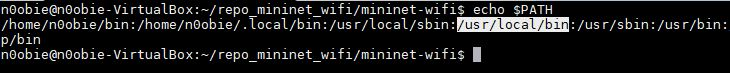
\includegraphics[width=\linewidth]{./img/util/1.JPG}
    \caption{PATH.}
  \label{fig:yo}
\end{figure}
\newline
Después de chequear el shellscript que se usa para la instalación y el Makefile en busca de alias se llego a la conclusión de que no se hacen uso de ellos y que se ejecuta el programa que esta en el siguiente Path.
\begin{figure}[!htb]
  \centering
    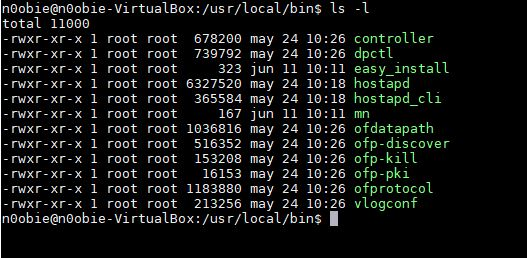
\includegraphics[width=0.8\linewidth]{./img/util/2.JPG}
    \caption{Ejecutable de Mininet}
  \label{fig:yo}
\end{figure}
\newline
Como se puede ver es el ejecutable de Mininet! De esta manera se puede comprobar que efectivamente Mininet-Wifi es un fork de Mininet, y que este engloba todas las características de Mininet. \newline
\newline
Cuando nosotros lanzamos Mininet-Wifi lo hacemos añadiendo un parámetro que es --wifi por lo que se espera que en este punto de entrada se trate los parametros con argsparse o similares para diferenciar cuando cargar Mininet original o cargar Mininet-Wifi. Accedemos al código para comprobarlo:\newpage
\begin{figure}[!htb]
  \centering
    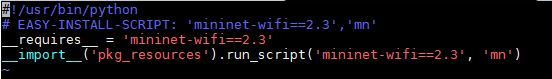
\includegraphics[width=0.8\linewidth]{./img/util/3.JPG}
    \caption{Entrypoint de Mininet-Wifi :)}
  \label{fig:yo}
\end{figure}
Sorpresa a que si? Como ya explicamos antes Mininet al igual que Mininet-Wifi está paquetizado por lo que este un simple warpper que carga de entre todos los paquetes el script \textbf{mn}, nombre \textbf{mininet-wifi}, versión \textbf{2.3} . \newline
\newline
Buscando y analizando se determinó que el script que se lanzaba reside en la siguiente ruta, y este si,  es el entrypoint de Mininet o Mininet-Wifi. Esto se ha deducido analizando una traza de llamadas al sistema con el comando \textbf{strace}. La traza se añade en los anexos de forma adicional.
\begin{figure}[!htb]
  \centering
    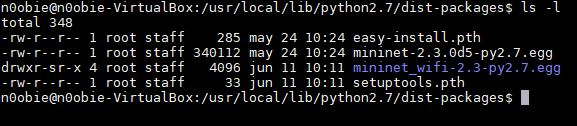
\includegraphics[width=0.8\linewidth]{./img/util/4.JPG}
    \caption{Mininet-Wifi paquetizado}
  \label{fig:yo}
\end{figure}
El script que carga se encuentra aquí:
\begin{figure}[!htb]
  \centering
    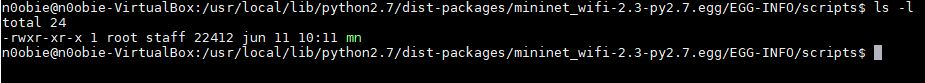
\includegraphics[width=\linewidth]{./img/util/5.JPG}
    \caption{Entrypoint de Mininet-Wifi}
  \label{fig:yo}
\end{figure}
\newline
Podemos ver como es el agente MininetRunner() quien gestiona los parámetros de entrada, crea la topología, levanta los nodos y los enlaces.
\begin{figure}[!htb]
  \centering
    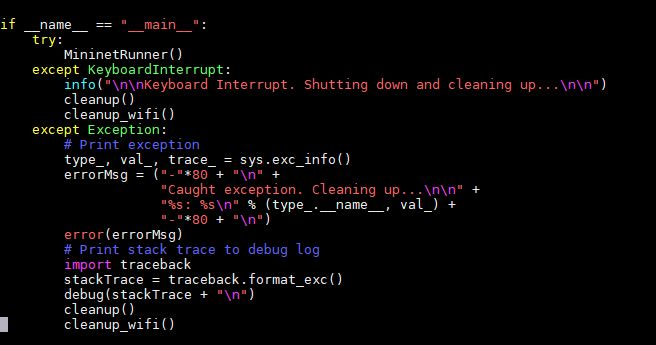
\includegraphics[width=0.8\linewidth]{./img/util/6.JPG}
    \caption{Entrypoint de Mininet-Wifi 2}
  \label{fig:yo}
\end{figure}

